% This file was created by matlab2tikz.
%
%The latest updates can be retrieved from
%  http://www.mathworks.com/matlabcentral/fileexchange/22022-matlab2tikz-matlab2tikz
%where you can also make suggestions and rate matlab2tikz.
%
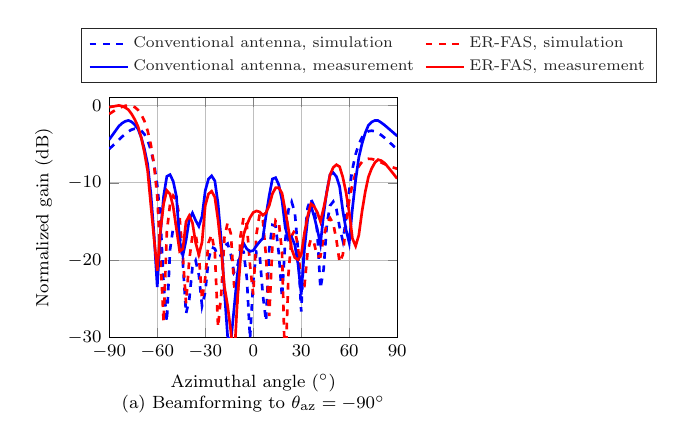
\begin{tikzpicture}[scale=0.8]

\begin{axis}[%
width=1.8in,
height=1.5in,
at={(0in,0in)},
scale only axis,
xmin=-90,
xmax=90,
xminorticks=true,
xtick={-90,-60,-30,0,30,60,90},
xlabel style={font=\color{white!15!black},font=\footnotesize,align=center},
xticklabel style = {font=\color{white!15!black},font=\footnotesize},
xlabel={ Azimuthal angle ($^\circ$) \\ (a) Beamforming to $\theta_\mathrm{az}=-90^\circ$},
ymin=-30,
ymax=1,
ytick={-30,-20,-10,0,10},
ylabel style={font=\color{white!15!black},font=\footnotesize},
yticklabel style = {font=\color{white!15!black},font=\footnotesize},
ylabel={Normalized gain (dB)},
axis background/.style={fill=white},
xmajorgrids,
xminorgrids,
ymajorgrids,
legend style={at={(1.9,1.06)}, anchor=south east, font=\scriptsize, legend cell align=left, align=left, draw=white!15!black, fill opacity=0.85}, legend columns=2
]
\addplot [color=blue, dashed, line width=1.2pt]
  table[row sep=crcr]{%
  -90	-5.61318	\\
-88	-5.2439	\\
-86	-4.85075	\\
-84	-4.44692	\\
-82	-4.04968	\\
-80	-3.68001	\\
-78	-3.36247	\\
-76	-3.12527	\\
-74	-3.00086	\\
-72	-3.02693	\\
-70	-3.24851	\\
-68	-3.72155	\\
-66	-4.51969	\\
-64	-5.74742	\\
-62	-7.56921	\\
-60	-10.28522	\\
-58	-14.58881	\\
-56	-23.05461	\\
-54	-27.92927	\\
-52	-18.64563	\\
-50	-15.7568	\\
-48	-15.27309	\\
-46	-16.65631	\\
-44	-20.28838	\\
-42	-26.886	\\
-40	-25.08804	\\
-38	-20.929	\\
-36	-20.03944	\\
-34	-21.88139	\\
-32	-25.89507	\\
-30	-24.10136	\\
-28	-20.00088	\\
-26	-18.30601	\\
-24	-18.50245	\\
-22	-19.53117	\\
-20	-19.37132	\\
-18	-18.1456	\\
-16	-17.84402	\\
-14	-19.25757	\\
-12	-21.57721	\\
-10	-20.88951	\\
-8	-18.86188	\\
-6	-18.90942	\\
-4	-22.32124	\\
-2	-30.11315	\\
0	-22.6948	\\
2	-18.89378	\\
4	-19.19959	\\
6	-24.49084	\\
8	-27.85979	\\
10	-18.53773	\\
12	-15.43121	\\
14	-15.57717	\\
16	-19.17722	\\
18	-24.79969	\\
20	-17.52947	\\
22	-13.50416	\\
24	-12.44316	\\
26	-13.83824	\\
28	-18.67886	\\
30	-26.6409	\\
32	-17.24194	\\
34	-13.2049	\\
36	-12.05169	\\
38	-12.9837	\\
40	-16.32742	\\
42	-23.65107	\\
44	-21.15109	\\
46	-15.39153	\\
48	-12.9536	\\
50	-12.42549	\\
52	-13.41662	\\
54	-15.75742	\\
56	-17.48149	\\
58	-14.68849	\\
60	-10.9661	\\
62	-8.21194	\\
64	-6.29731	\\
66	-4.98957	\\
68	-4.12754	\\
70	-3.60187	\\
72	-3.33443	\\
74	-3.26625	\\
76	-3.3507	\\
78	-3.54958	\\
80	-3.83087	\\
82	-4.16747	\\
84	-4.53652	\\
86	-4.91919	\\
88	-5.3006	\\
90	-5.66995	\\
};
\addlegendentry{Conventional antenna, simulation}

\addplot [color=red, dashed, line width=1.2pt]
  table[row sep=crcr]{%
  -90	-1.11386	\\
  -88	-0.83527	\\
  -86	-0.58154	\\
  -84	-0.35859	\\
  -82	-0.17669	\\
  -80	-0.05063	\\
  -78	-2.57E-06	\\
  -76	-0.0497	\\
  -74	-0.2309	\\
  -72	-0.5829	\\
  -70	-1.15635	\\
  -68	-2.01945	\\
  -66	-3.27016	\\
  -64	-5.06317	\\
  -62	-7.67944	\\
  -60	-11.75918	\\
  -58	-19.62042	\\
  -56	-27.98482	\\
  -54	-16.29905	\\
  -52	-12.76648	\\
  -50	-11.66132	\\
  -48	-12.21637	\\
  -46	-14.51907	\\
  -44	-19.42067	\\
  -42	-25.547	\\
  -40	-19.96604	\\
  -38	-16.818	\\
  -36	-16.62836	\\
  -34	-19.23068	\\
  -32	-25.05116	\\
  -30	-22.27459	\\
  -28	-17.75878	\\
  -26	-16.69887	\\
  -24	-18.95752	\\
  -22	-28.63013	\\
  -20	-24.37422	\\
  -18	-17.06474	\\
  -16	-15.14657	\\
  -14	-16.5587	\\
  -12	-23.13089	\\
  -10	-25.87283	\\
  -8	-16.92338	\\
  -6	-14.45824	\\
  -4	-15.43014	\\
  -2	-20.6587	\\
  0	-24.43235	\\
  2	-16.64525	\\
  4	-14.06242	\\
  6	-14.8129	\\
  8	-19.52277	\\
  10	-27.202	\\
  12	-18.01607	\\
  14	-14.80542	\\
  16	-15.08498	\\
  18	-18.99065	\\
  20	-35.04671	\\
  22	-21.81758	\\
  24	-16.86096	\\
  26	-16.10877	\\
  28	-18.22787	\\
  30	-23.30928	\\
  32	-23.32981	\\
  34	-18.90999	\\
  36	-17.26372	\\
  38	-17.77267	\\
  40	-19.47274	\\
  42	-19.50922	\\
  44	-17.12606	\\
  46	-15.19294	\\
  48	-14.54594	\\
  50	-15.24913	\\
  52	-17.37578	\\
  54	-20.26055	\\
  56	-19.28749	\\
  58	-15.3562	\\
  60	-12.26569	\\
  62	-10.1607	\\
  64	-8.75647	\\
  66	-7.84734	\\
  68	-7.29521	\\
  70	-7.00226	\\
  72	-6.89538	\\
  74	-6.91808	\\
  76	-7.02617	\\
  78	-7.18541	\\
  80	-7.36982	\\
  82	-7.56035	\\
  84	-7.74358	\\
  86	-7.91059	\\
  88	-8.05606	\\
  90	-8.1777	\\  
};
\addlegendentry{ER-FAS, simulation}

\addplot [color=blue, line width=1.2pt]
  table[row sep=crcr]{%
  -90	-4.4099	\\
-88	-3.83308	\\
-86	-3.25626	\\
-84	-2.67944	\\
-82	-2.30453	\\
-80	-2.05671	\\
-78	-1.93597	\\
-76	-2.12002	\\
-74	-2.49323	\\
-72	-3.05559	\\
-70	-4.13782	\\
-68	-5.64586	\\
-66	-7.57972	\\
-64	-11.36576	\\
-62	-16.65423	\\
-60	-23.44513	\\
-58	-16.46276	\\
-56	-11.70182	\\
-54	-9.16232	\\
-52	-8.94062	\\
-50	-9.80615	\\
-48	-11.7589	\\
-46	-17.49971	\\
-44	-19.38677	\\
-42	-17.42006	\\
-40	-14.75029	\\
-38	-13.89299	\\
-36	-14.84814	\\
-34	-15.61079	\\
-32	-14.33764	\\
-30	-11.02868	\\
-28	-9.52636	\\
-26	-9.096	\\
-24	-9.73762	\\
-22	-12.68062	\\
-20	-17.46048	\\
-18	-24.07718	\\
-16	-29.85473	\\
-14	-30.58478	\\
-12	-26.26733	\\
-10	-21.97854	\\
-8	-19.16128	\\
-6	-17.81554	\\
-4	-18.53937	\\
-2	-18.84916	\\
0	-18.74491	\\
2	-18.13407	\\
4	-17.61077	\\
6	-17.175	\\
8	-14.20168	\\
10	-11.64085	\\
12	-9.49251	\\
14	-9.33613	\\
16	-10.26062	\\
18	-12.26598	\\
20	-15.74745	\\
22	-17.32692	\\
24	-17.00438	\\
26	-18.02316	\\
28	-20.49384	\\
30	-24.41642	\\
32	-18.55065	\\
34	-14.71325	\\
36	-12.90425	\\
38	-14.29409	\\
40	-15.96157	\\
42	-17.9067	\\
44	-14.06508	\\
46	-11.08111	\\
48	-8.95483	\\
50	-8.68417	\\
52	-9.19161	\\
54	-10.47717	\\
56	-13.61227	\\
58	-16.03724	\\
60	-17.75209	\\
62	-13.32805	\\
64	-9.64647	\\
66	-6.70734	\\
68	-4.9371	\\
70	-3.55442	\\
72	-2.5593	\\
74	-2.14553	\\
76	-1.94356	\\
78	-1.95338	\\
80	-2.21667	\\
82	-2.52518	\\
84	-2.87892	\\
86	-3.23563	\\
88	-3.59234	\\
90	-3.94905	\\
};
\addlegendentry{Conventional antenna, measurement }

\addplot [color=red, line width=1.2pt]
  table[row sep=crcr]{%
  -90	-0.22568	\\
-88	-0.15046	\\
-86	-0.07523	\\
-84	0	\\
-82	-0.08694	\\
-80	-0.27393	\\
-78	-0.56096	\\
-76	-1.10635	\\
-74	-1.82929	\\
-72	-2.7298	\\
-70	-4.16899	\\
-68	-6.07643	\\
-66	-8.4521	\\
-64	-12.86944	\\
-62	-17.16614	\\
-60	-21.3422	\\
-58	-16.1464	\\
-56	-12.69519	\\
-54	-10.98857	\\
-52	-11.45876	\\
-50	-13.10906	\\
-48	-15.93947	\\
-46	-18.84217	\\
-44	-18.53865	\\
-42	-15.0289	\\
-40	-14.24651	\\
-38	-15.14989	\\
-36	-17.73903	\\
-34	-19.27063	\\
-32	-17.67478	\\
-30	-12.95146	\\
-28	-11.44766	\\
-26	-11.07956	\\
-24	-11.84718	\\
-22	-14.8036	\\
-20	-18.66325	\\
-18	-23.42613	\\
-16	-25.86403	\\
-14	-29.18241	\\
-12	-33.38128	\\
-10	-25.45006	\\
-8	-19.88113	\\
-6	-16.67449	\\
-4	-15.43071	\\
-2	-14.48197	\\
0	-13.82827	\\
2	-13.63023	\\
4	-13.7486	\\
6	-14.18339	\\
8	-13.85954	\\
10	-12.93041	\\
12	-11.39601	\\
14	-10.63955	\\
16	-10.62295	\\
18	-11.34619	\\
20	-13.55916	\\
22	-15.95697	\\
24	-18.53963	\\
26	-19.67349	\\
28	-19.92595	\\
30	-19.29701	\\
32	-16.49703	\\
34	-14.30484	\\
36	-12.72045	\\
38	-13.02902	\\
40	-13.78572	\\
42	-14.99056	\\
44	-13.26447	\\
46	-11.25735	\\
48	-8.9692	\\
50	-8.01091	\\
52	-7.66021	\\
54	-7.91709	\\
56	-9.28088	\\
58	-11.24723	\\
60	-13.81613	\\
62	-17.18445	\\
64	-18.16187	\\
66	-16.74836	\\
68	-13.68448	\\
70	-11.17956	\\
72	-9.23362	\\
74	-8.15061	\\
76	-7.40589	\\
78	-6.99947	\\
80	-7.12952	\\
82	-7.42943	\\
84	-7.89917	\\
86	-8.41677	\\
88	-8.93437	\\
90	-9.45197	\\
};
\addlegendentry{ER-FAS, measurement}

\end{axis}

\end{tikzpicture}%